\documentclass[11pt]{article}
\usepackage{geometry} % Pour passer au format A4
\geometry{hmargin=1cm, vmargin=1cm} % 

% Page et encodage
\usepackage[T1]{fontenc} % Use 8-bit encoding that has 256 glyphs
\usepackage[english,french]{babel} % Français et anglais
\usepackage[utf8]{inputenc} 

\usepackage{lmodern}
\setlength\parindent{0pt}

% Graphiques
\usepackage{graphicx,float,grffile}

% Maths et divers
\usepackage{amsmath,amsfonts,amssymb,amsthm,verbatim}
\usepackage{multicol,enumitem,url,eurosym,gensymb}

% Sections
\usepackage{sectsty} % Allows customizing section commands
\allsectionsfont{\centering \normalfont\scshape}

% Tête et pied de page

\usepackage{fancyhdr} 
\pagestyle{fancyplain} 

\fancyhead{} % No page header
\fancyfoot{}

\renewcommand{\headrulewidth}{0pt} % Remove header underlines
\renewcommand{\footrulewidth}{0pt} % Remove footer underlines

\newcommand{\horrule}[1]{\rule{\linewidth}{#1}} % Create horizontal rule command with 1 argument of height

%----------------------------------------------------------------------------------------
%	Début du document
%----------------------------------------------------------------------------------------

\begin{document}

%----------------------------------------------------------------------------------------
% RE-DEFINITION
%----------------------------------------------------------------------------------------
% MATHS
%-----------

\newtheorem{Definition}{Définition}
\newtheorem{Theorem}{Théorème}
\newtheorem{Proposition}{Propriété}

% MATHS
%-----------
\renewcommand{\labelitemi}{$\bullet$}
\renewcommand{\labelitemii}{$\circ$}
%----------------------------------------------------------------------------------------
%	Titre
%----------------------------------------------------------------------------------------

\setlength{\columnseprule}{1pt}

\textbf{Nom, Prénom :} \hspace{8cm} \textbf{Classe :} \hspace{3cm} \textbf{Date :}\\
\vspace{-0.8cm}
\begin{center}
  \textit{If you do the work, you get rewarded. There are no shortcuts in life.}  - \textbf{Michael Jordan}
\end{center}
\vspace{-0.8cm}

\subsection*{Équations}
\begin{multicols}{2}\noindent
  \begin{enumerate}
  \item[a.)] $-2x + 5 = 9$
  \item[b.)] $x - 10 = -11$
  \item[c.)] $-3x - 2 = 3x + 34$
  \item[d.)] $4x + 10 = -4x + 18$
    \end{enumerate}
\end{multicols}

\vspace{-0.4cm}
\horrule{1px}
\vspace{-0.8cm}

\begin{multicols}{2}

\subsubsection*{Problème 1 - Vase}

Antoine crée des objets de décoration avec des vases, des billes et de l’eau colorée. Pour sa nouvelle création, il décide d’utiliser le vase et les billes ayant les caractéristiques suivantes :

\textbf{Il met 150 billes dans le vase. Peut-il ajouter un litre d’eau colorée sans risquer le débordement ?}

Rappels : 

\begin{itemize}
\item Volume de la sphère = $\dfrac{4}{3} \times \pi  \times rayon^3$
\end{itemize}

\begin{figure}[H]
      \centering
      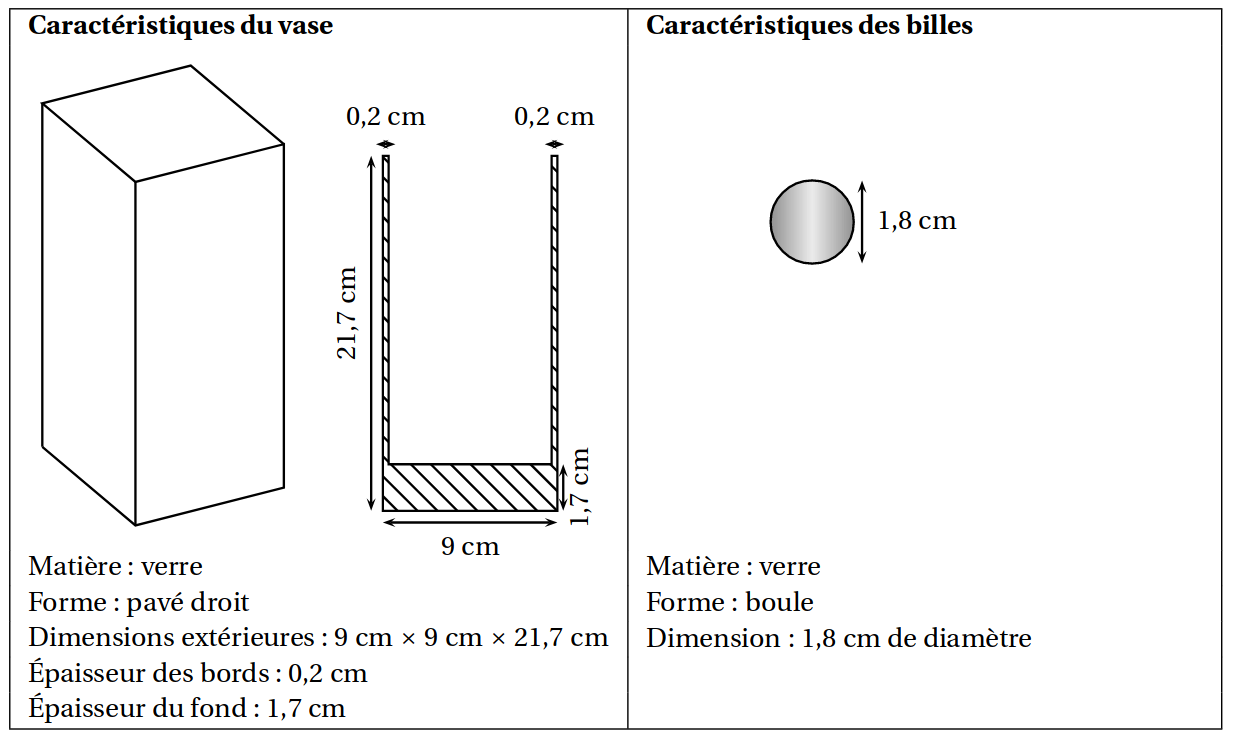
\includegraphics[width=\linewidth]{3x3-volumes-1/sources/bille.png}
\end{figure}

\end{multicols}

\begin{multicols}{2}

\subsubsection*{Problème 2 - Sel}

La fleur de sel est la mince couche de cristaux blancs qui se forme et affleure la surface des marais salants. Chaque soir, Jean cueille la fleur de sel à la surface des carreaux. Pour transporter sa récolte, il utilise une brouette comme sur le schéma ci-dessous.

\begin{enumerate}
\item Montrer que cette brouette a un volume de 77 litres.
\item Sachant que 1 litre de fleur de sel pèse 900 grammes, calculer la masse en kg du contenu d’une brouette remplie de fleur de sel
\end{enumerate}

\begin{figure}[H]
      \centering
      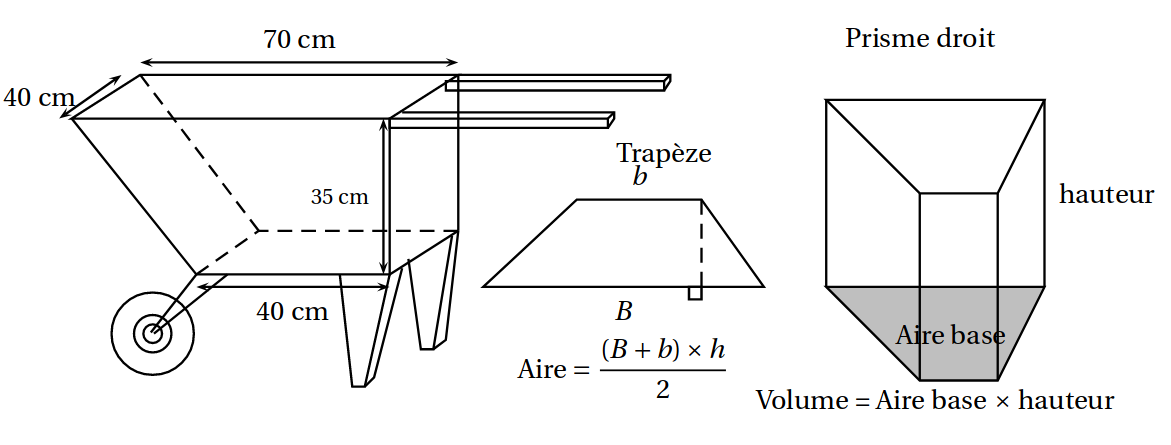
\includegraphics[width=\linewidth]{3x3-volumes-1/sources/brouette.png}
\end{figure}

\end{multicols}

\subsubsection*{Problème 3 - Yourte}

Samia vit dans un appartement dont la surface au sol est de $35 m^2$. Elle le compare avec une yourte, l’habitat traditionnel mongol

\begin{figure}[H]
      \centering
      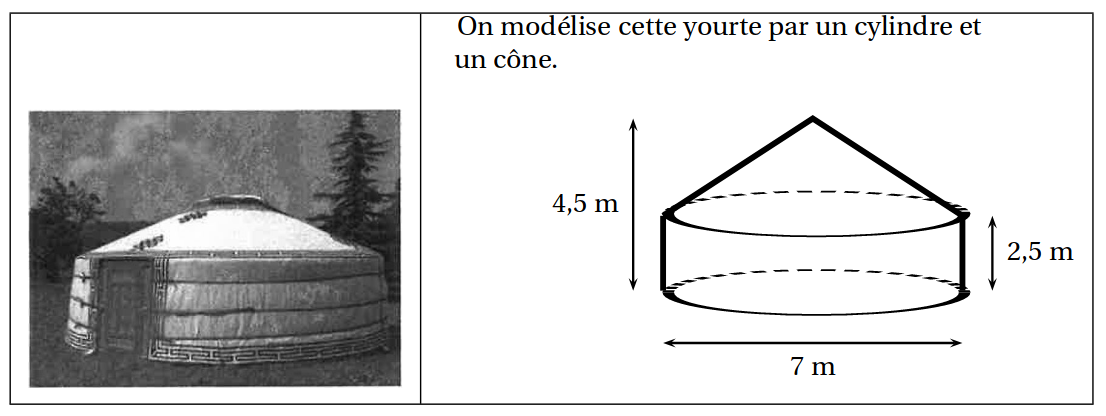
\includegraphics[width=0.6\linewidth]{3x3-volumes-1/sources/yourte.png}
\end{figure}

\begin{enumerate}
\item Montrer que l’appartement de Samia offre une plus petite surface au sol que celle de la yourte.
\item Calculer le volume de la yourte en m3.
\end{enumerate}
  
Rappels : 

\begin{itemize}
  \item Aire du disque = $\pi \times rayon^2$
  \item Volume du cylindre = $\pi \times rayon^2 \times hauteur$
  \item Volume du cône = $\dfrac{1}{3} \times \pi \times rayon^2 \times hauteur$
\end{itemize}

\begin{multicols}{2}

\subsubsection*{Problème 4 - Escalier}

  Afin de faciliter l'accès à sa piscine, Monsieur Joseph décide de construire un escalier constitué de deux prismes superposés dont les bases sont des triangles rectangles.

  \begin{enumerate}
  \item Démontrer que le volume de l'escalier est égal à $1,26 m^3$.
  \item Sachant que l'escalier est un ouvrage en béton courant, déterminer le nombre de sacs de ciment de 35 kg nécessaires à la réalisation de l'escalier.
  \item Déterminer la quantité d'eau nécessaire à cet ouvrage.
  \end{enumerate}

  \begin{figure}[H]
        \centering
        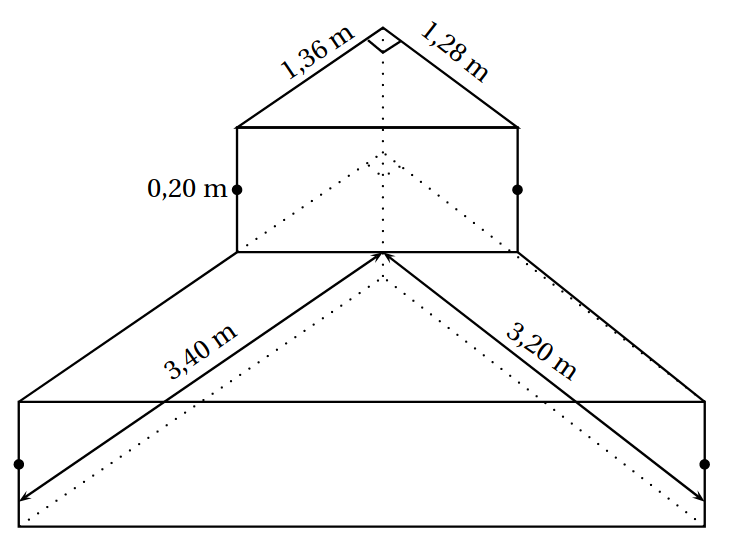
\includegraphics[width=\linewidth]{3x3-volumes-1/sources/escalier.png}
  \end{figure}


\end{multicols}

\textbf{Information 1 :} Volume du prisme = aire de la base $\times$ hauteur ;\quad  1~L = 1~dm$^3$

\textbf{Information 2 :} Voici la reproduction d'une étiquette figurant au dos d'un sac de ciment
de 35~kg.

\begin{center}
  \begin{tabular}{|c|c|c|c|c|}  \hline
    Dosage pour 1 sac de 35 kg	&Volume de béton obtenu	&Sable (seaux)	&Gravillons (seaux)	&Eau\\ \hline
    Mortier courant 			&105 L					&10				&					&16 L\\ \hline
    Ouvrages en béton courant	&100 L					&5				&8 					&17 L\\ \hline
    Montage de murs 			&120 L 					&12				&					&18~L\\ \hline
  \end{tabular}
\end{center}
\textit{Dosages donnés à titre indicatif et pouvant varier suivant les matériaux régionaux et le taux d'hygrométrie des granulats}



\subsection*{Volumes de la vie courante}


\end{document}
